
I begin by validating the log-normality assumption at the tract level. Figure \ref{fig:median} examines the fit for median income, comparing observed values with those predicted under log-normality for each census tract, where observations are grouped into equal-sized bins using binscatter methods.\footnote{See \cite{cattaneo}.} The relationship is remarkably strong ($\beta$ = 0.98, $R^2$ = 0.98), with predicted values differing from observed ones by just 4.6\% on average. The near-unit slope coefficient and $R^2$ indicate that log-normality captures the central tendency of the income distribution particularly well.

Figure \ref{fig:median} shows the relationship for the P80/P20 ratio. The regression yields a slope coefficient of 0.75 ($R^2$ = 0.81), with predicted values deviating from observed ones by 5\% on average. Consistent with the fact that real income distributions tend to have heavier tails, the coefficient below unity suggests that the log-normal distribution slightly underestimates inequality.

Next, I show how the mixture approach generates substantial differences between the distribution implied solely by tract means -- where everyone within a tract is assumed to have the same income -- and the estimated individual-level distribution. Figure \ref{fig:distributions} plots both distributions for net equivalised income in 2022. The tract-level distribution (in dark blue) exhibits higher kurtosis and is more concentrated around its mode of approximately €20,000, as it collapses all within-tract variation to a single point. In contrast, the estimated individual distribution shows greater dispersion and a lower mode, reflecting the within-tract inequality captured by the mixture of log-normal local distributions. The heavier left tail and more gradual right tail of the mixture distribution suggest that a simple aggregation of tract means would vastly understate income inequality, particularly by failing to account for the substantial mass of low-income households and the long right tail of high earners.

\begin{figure}[H]
\begin{center}
\captionsetup{justification=centering}
\caption{Validation of log-normality: median income}
\label{fig:median}
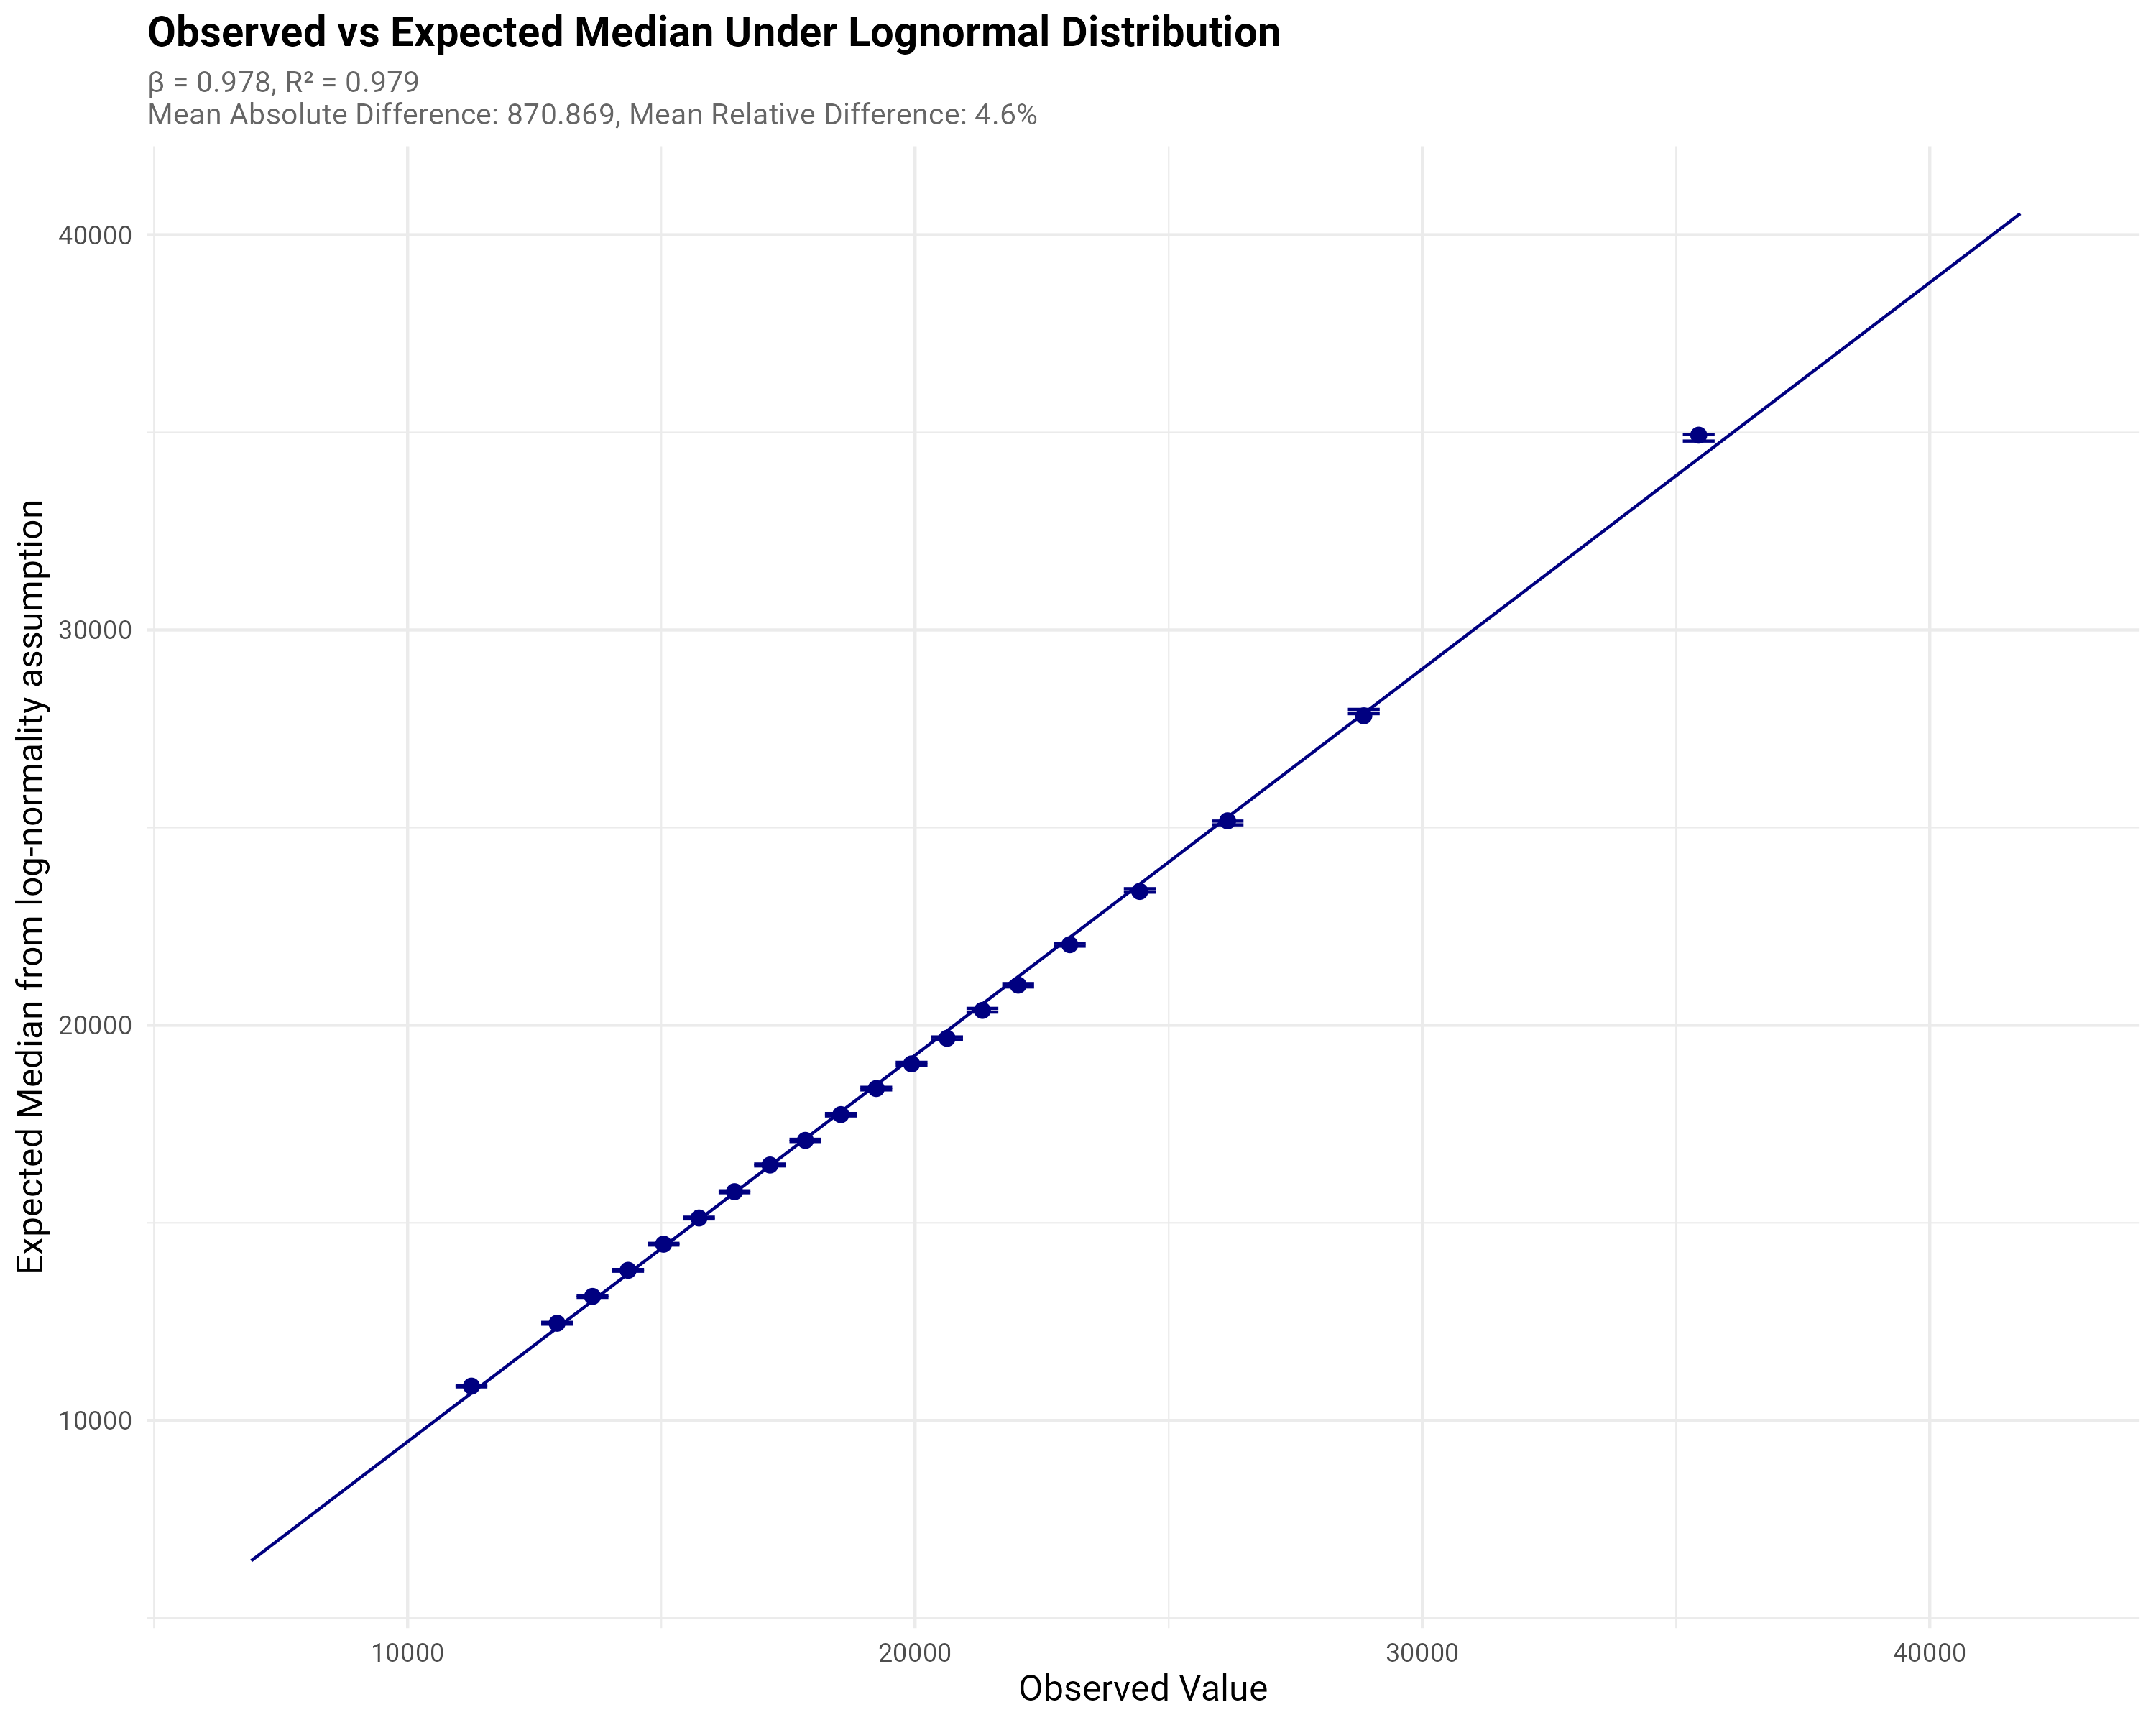
\includegraphics[width=0.75\textwidth]{output/binned_scatter_median.png}
\end{center}
\begin{fignotes2}
\textbf{Notes:} This figure shows a binned scatter plot comparing observed median income with predicted values under the log-normal assumption for each census tract. Source: Spanish Statistical Office and author's calculations.
\end{fignotes2}
\end{figure}

\begin{figure}[H]
\begin{center}
\captionsetup{justification=centering}
\caption{Validation of log-normality: P80/P20 ratio}
\label{fig:p80p20}
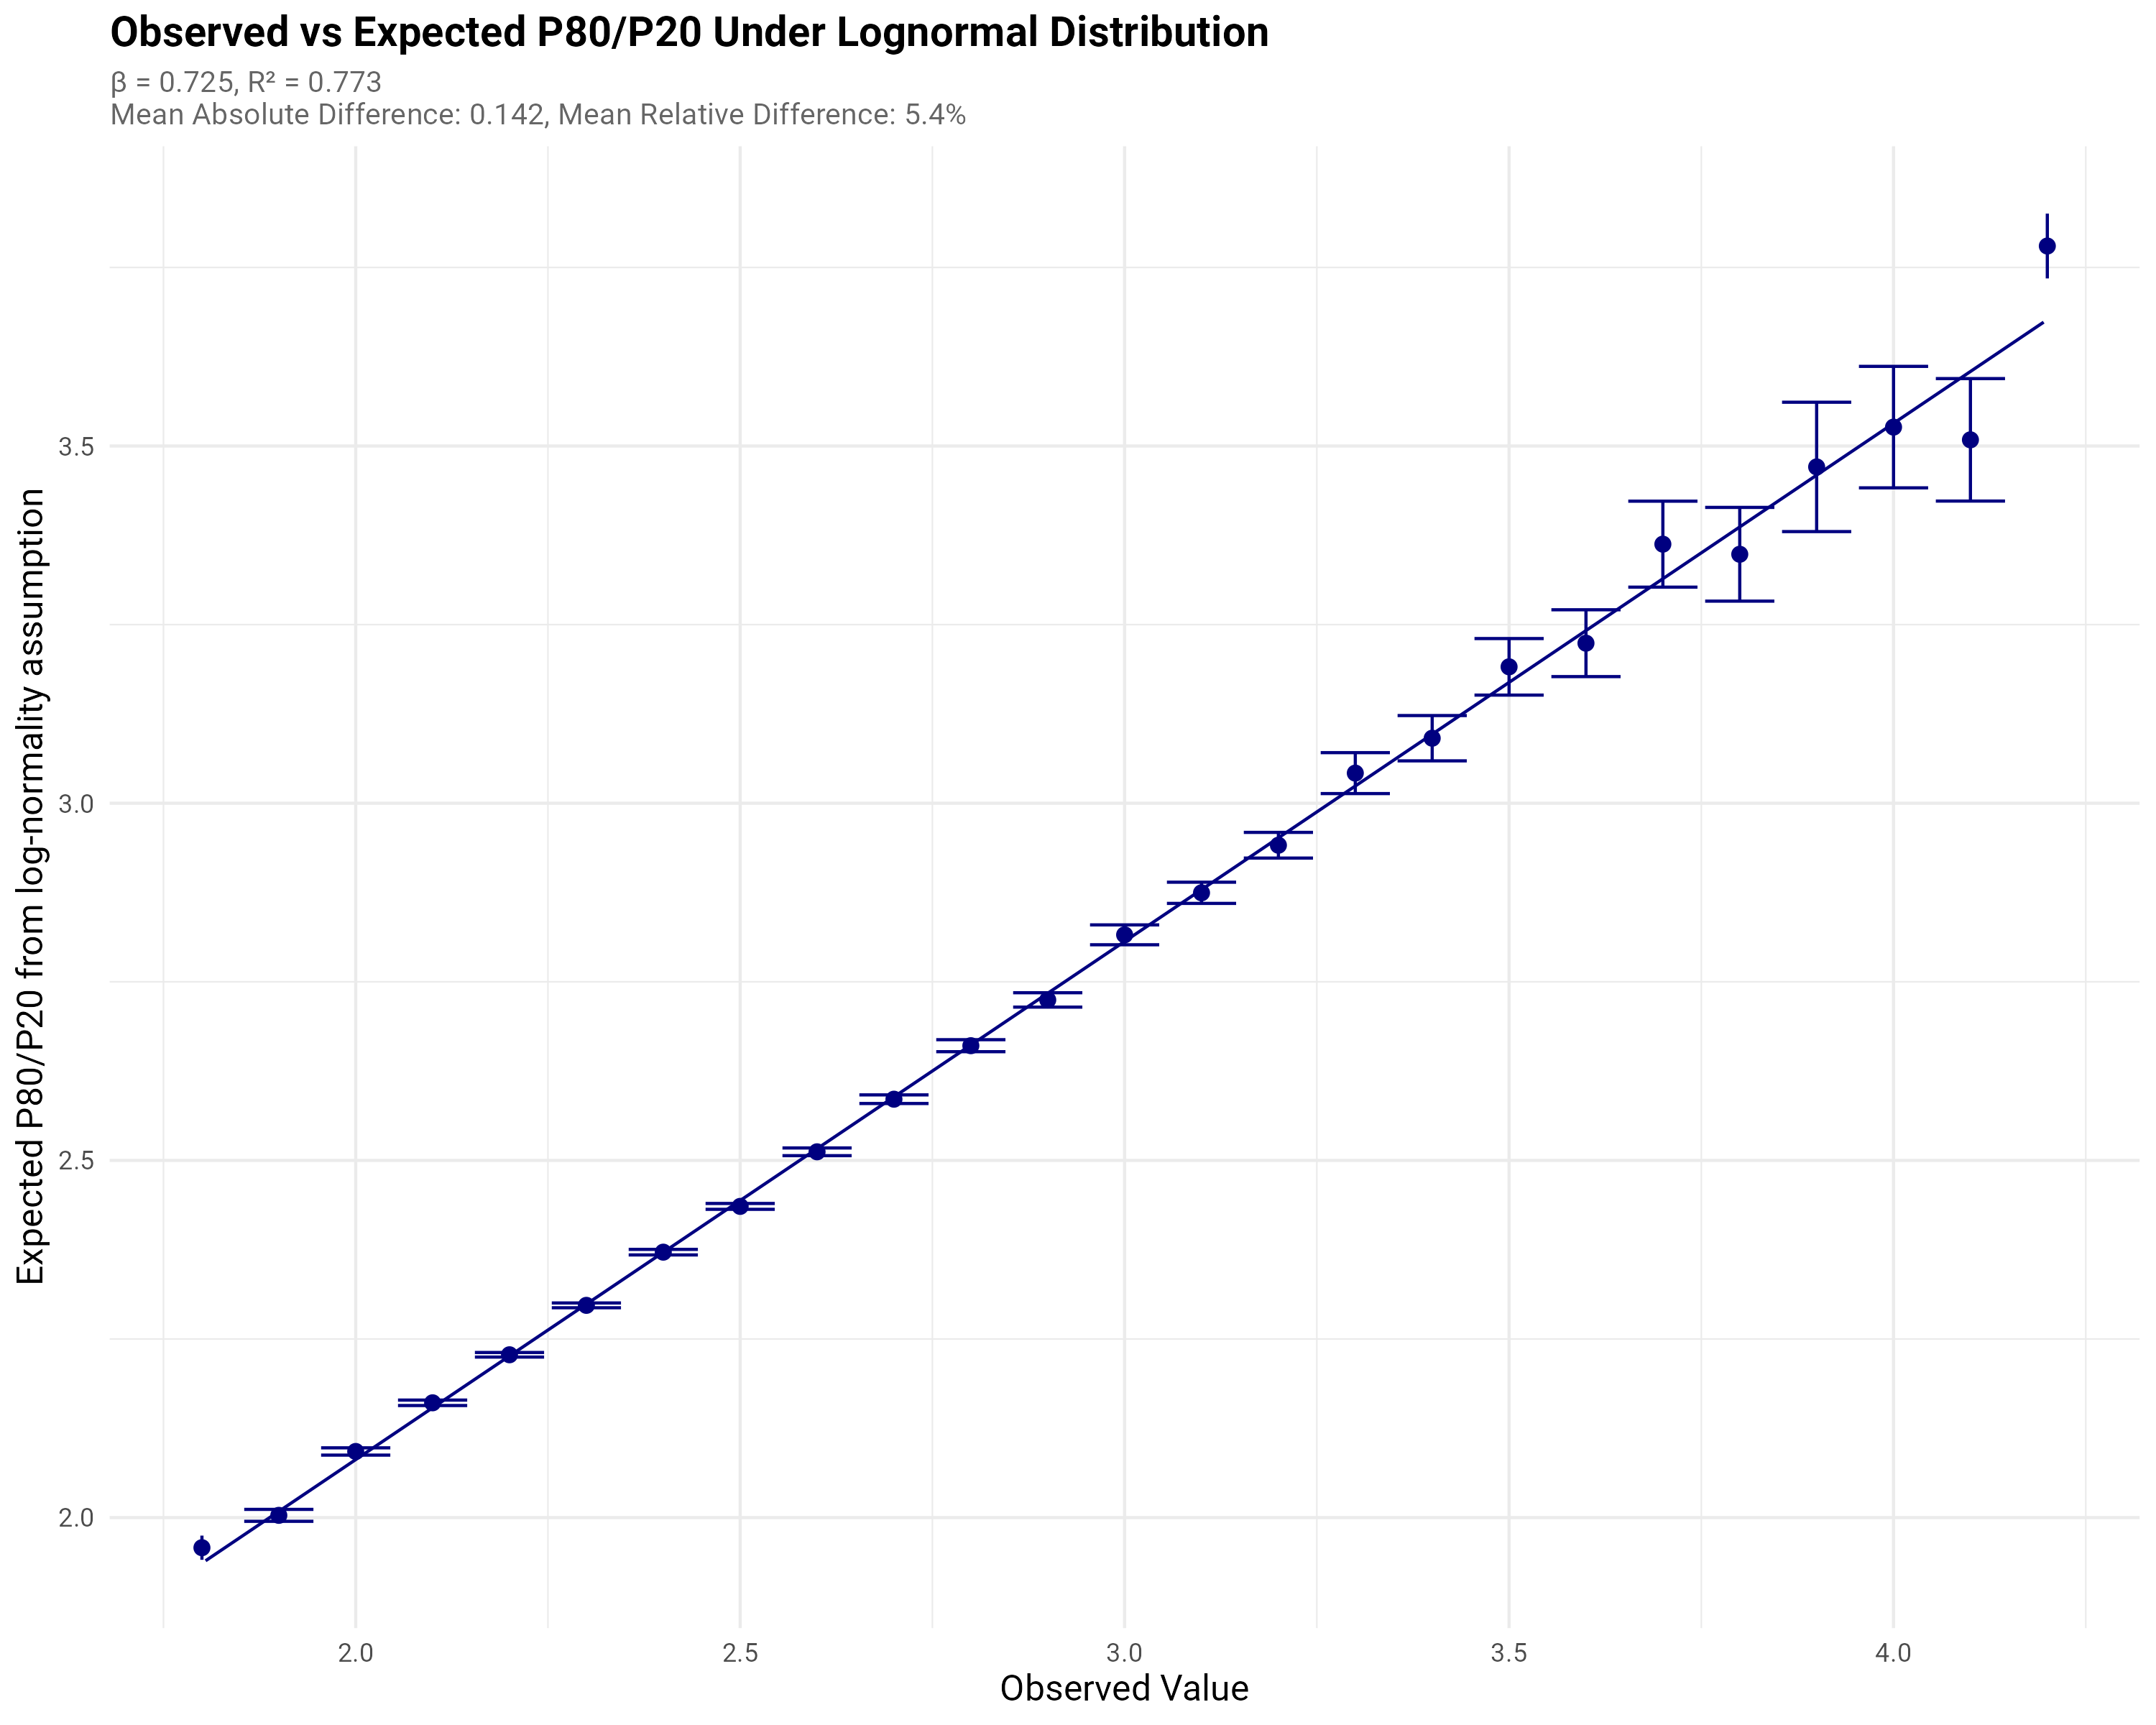
\includegraphics[width=0.75\textwidth]{output/binned_scatter_p80p20.png}
\end{center}
\begin{fignotes2}
\textbf{Notes:} This figure shows a binned scatter plot comparing observed P80/P20 ratios with predicted values under the log-normal assumption for each census tract. Source: Spanish Statistical Office and author's calculations.
\end{fignotes2}
\end{figure}

\begin{figure}[H]
\begin{center}
\captionsetup{justification=centering}
\caption{Estimated mixture vs. tract means}
\label{fig:distributions}
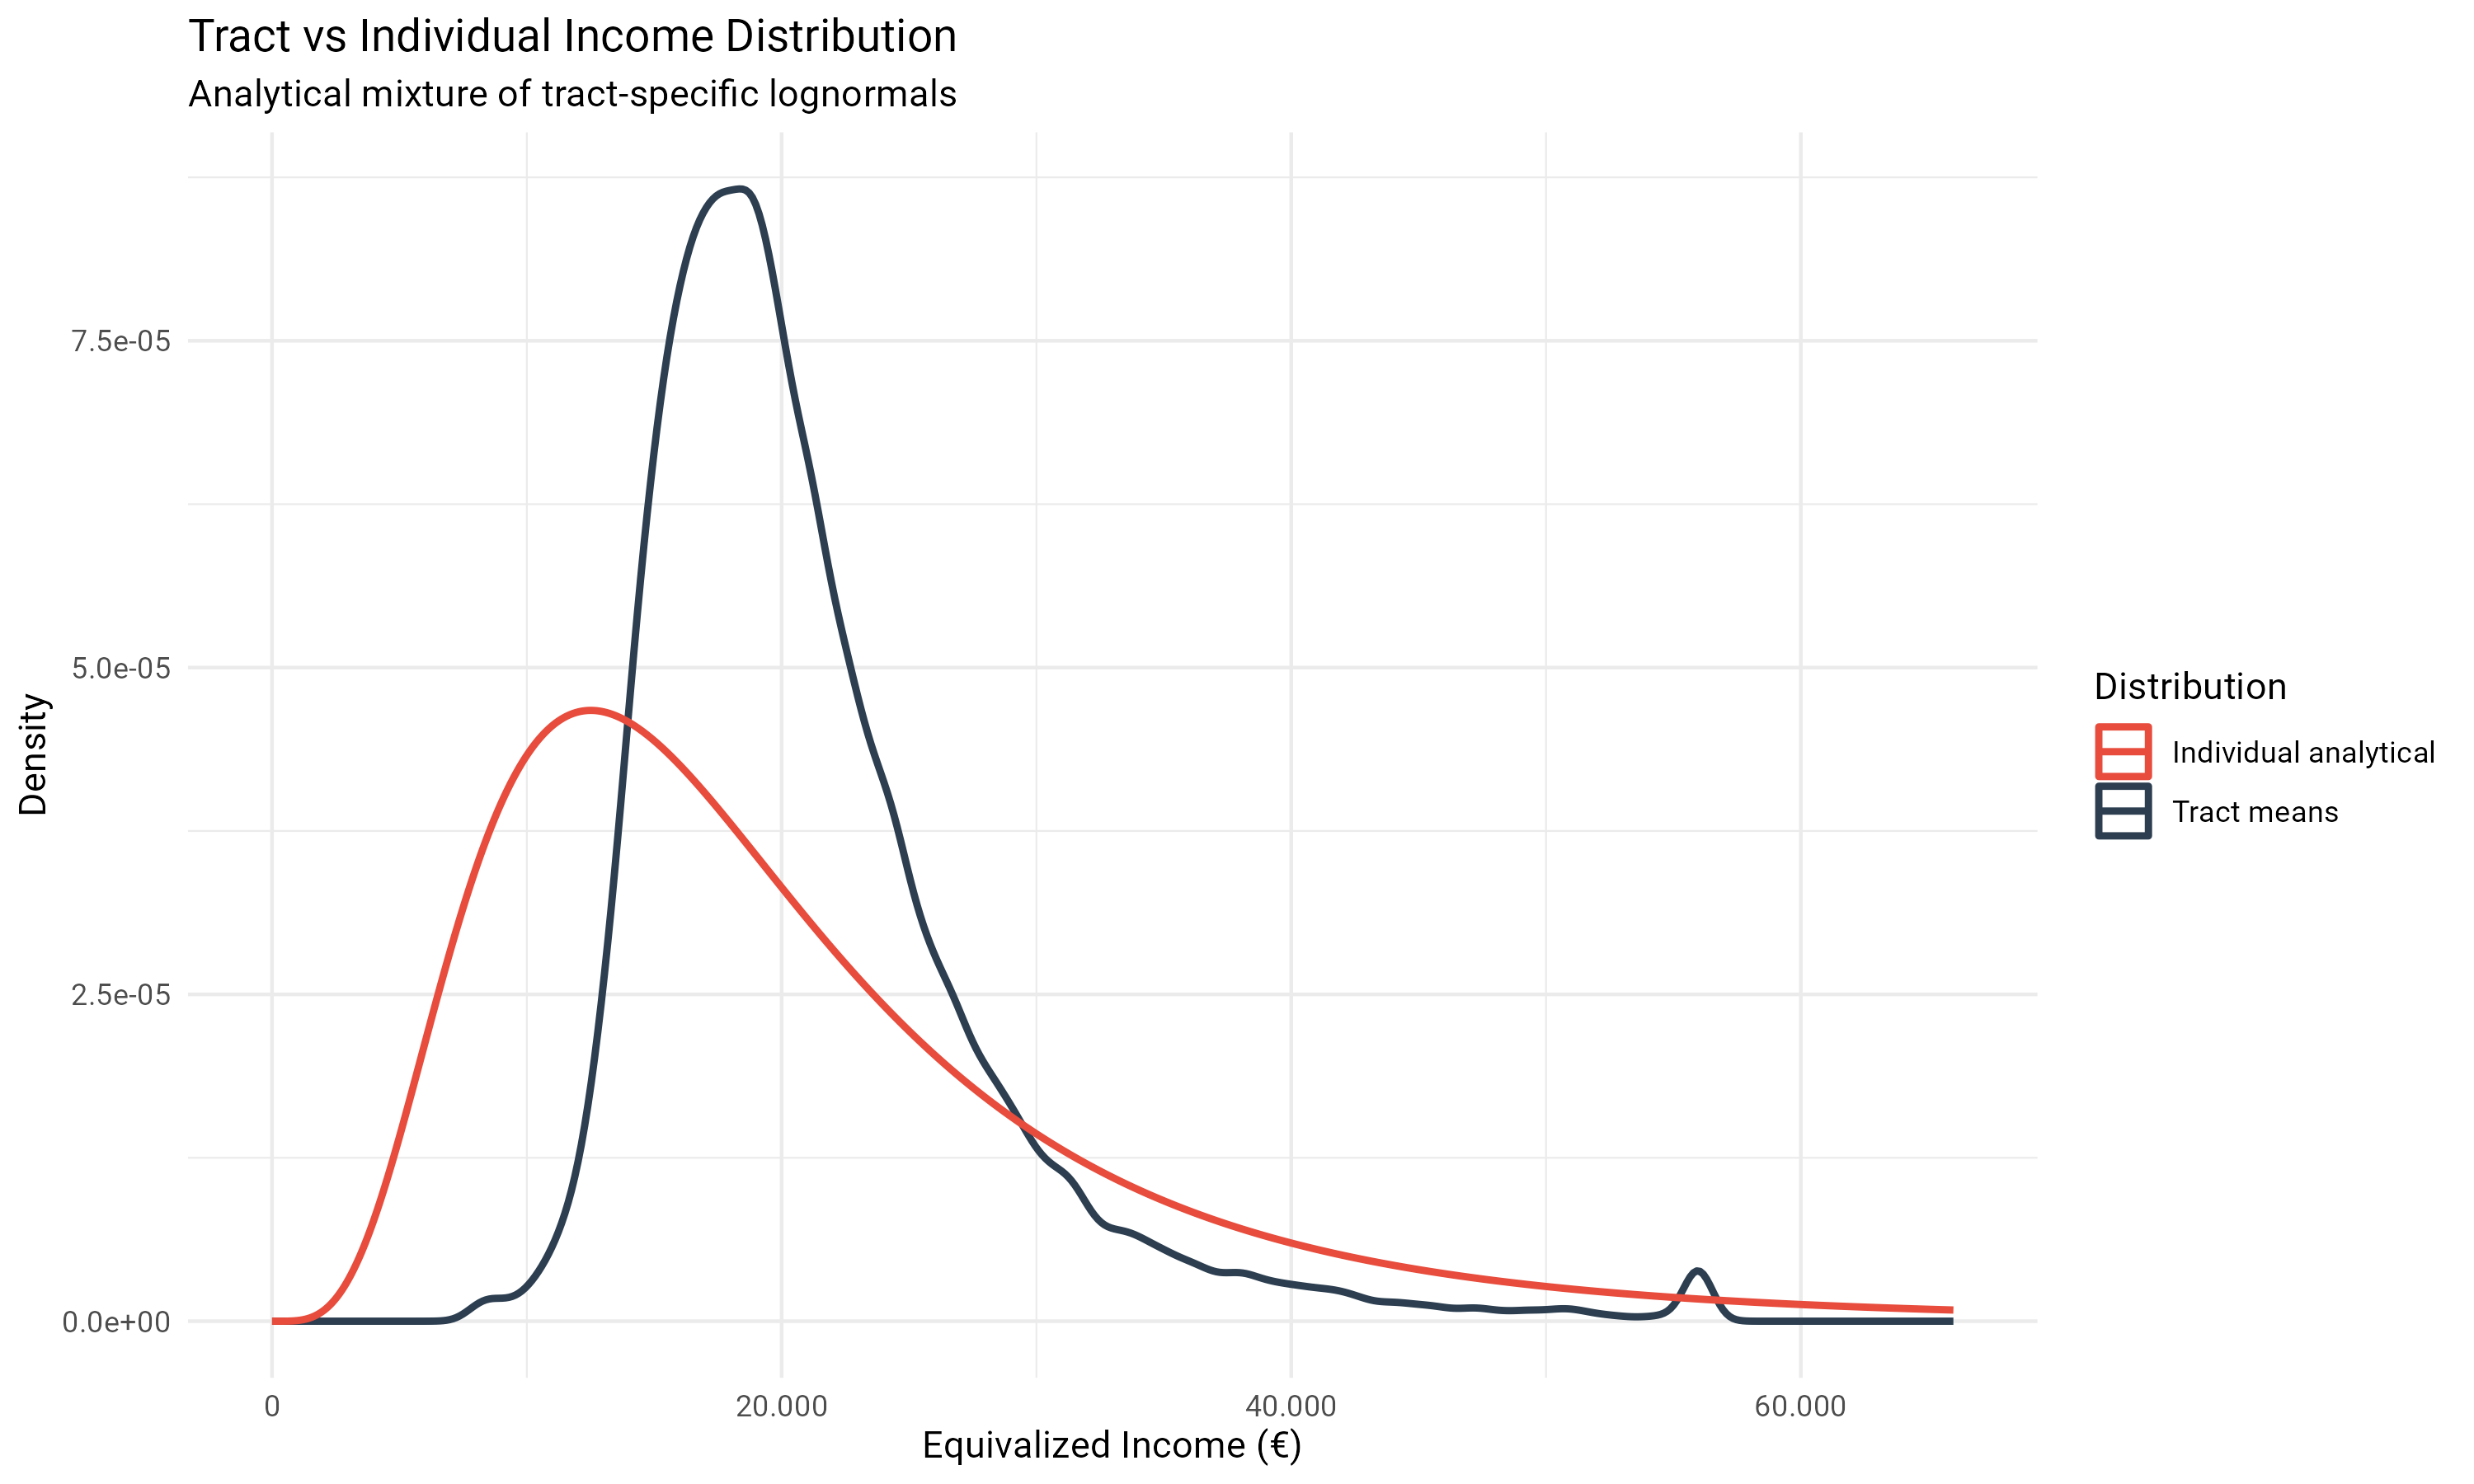
\includegraphics[width=0.75\textwidth]{output/tract_vs_individual_income_distribution.png}
\end{center}
\begin{fignotes2}
\textbf{Notes:} This figure shows two approaches to approximating the individual income distribution: using tract means (in dark blue), where everyone within a tract is assumed to have the same income, and using a mixture of log-normals (in red) that incorporates within-tract inequality. The tract means distribution is calculated as a population-weighted kernel density of tract means. The mixture distribution is constructed using tract-specific log-normal distributions, where the parameters of each component are derived from observed tract means and Gini coefficients, and mixture weights correspond to tract population shares. Source: Spanish Statistical Office and author's calculations.
\end{fignotes2}
\end{figure}

A natural question arises: to what extent does the mixture of local-level distributions improve the accuracy of measuring the income distribution compared to simply assuming log-normality at the national level? The comparison shown in Figure \ref{fig:dist2} suggests that the improvement is arguably limited. The national log-normal distribution -- derived using the population-weighted mean equivalised income and Gini index across all tracts -- tends to overestimate incomes at the lower end of the distribution and underestimate incomes at the upper tail, but it provides a reasonably close approximation to the mixture of tract-level distributions. These results suggest that, in contexts where more granular data is not available, assuming log-normality at the national level might remain a fair approximation for capturing the overall shape of the income distribution, though with some loss in precision. This is consistent with previous evidence showing that log-normal densities approximate very well the empirical distribution of per capita income in large cross-country panels \citep{lopez2006normal}.

%Indeed, the mixture approach appears to perform notably better at capturing key distributional statistics. For instance, the median income from the mixture distribution (€19,290) almost exactly matches the official median from the 2022 Survey of Living Conditions (€19,160), while the national log-normal approximation yields a lower accurate estimate of €18,297. 

\begin{figure}[H]
\begin{center}
\captionsetup{justification=centering}
\caption{Estimated mixture vs. national log-normal}\label{fig:dist2}
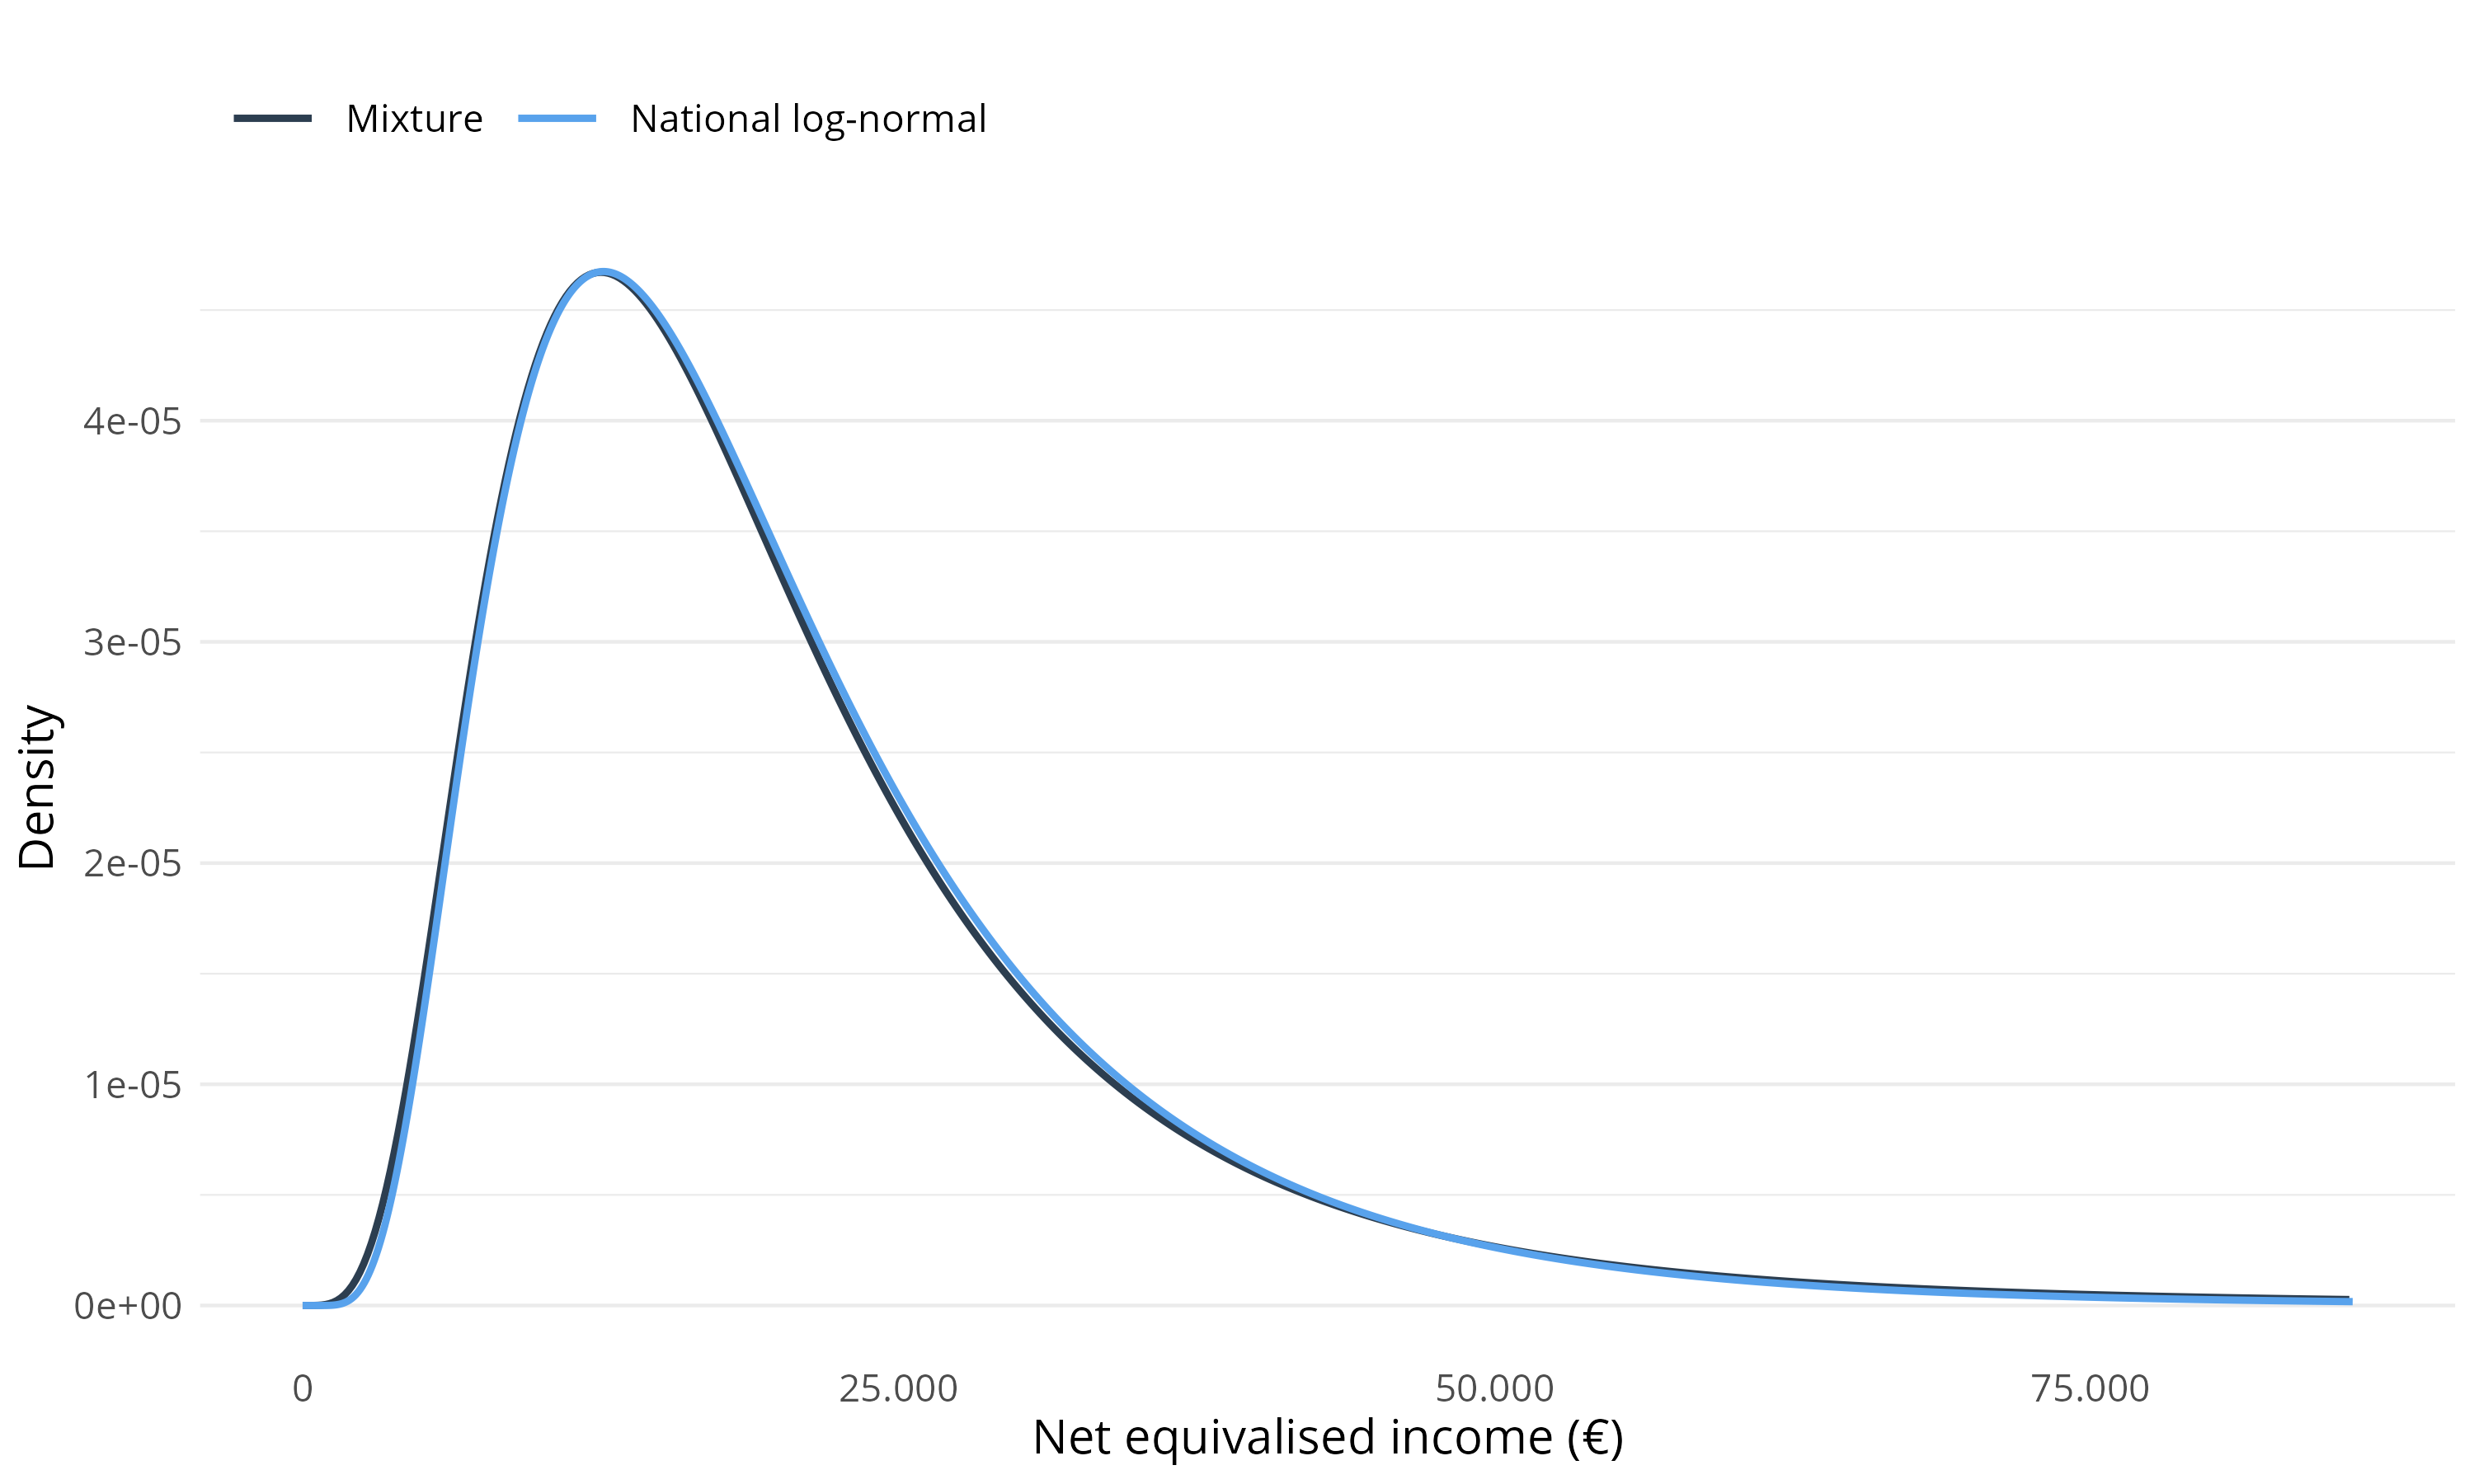
\includegraphics[width=0.75\textwidth]{output/tract_vs_national_income_distribution.png}
\end{center}
\begin{fignotes2}
\textbf{Notes:} This figure compares the income distribution derived from a mixture of tract-level log-normal distributions (navy) with a single national-level log-normal distribution (light blue). The mixture distribution is constructed using tract-specific log-normal distributions, where the parameters of each component are derived from observed tract means and Gini coefficients, and mixture weights correspond to tract population shares. The parameters for the national log-normal are given by the population-weighted mean equivalised income and Gini index across all tracts. Source: Spanish Statistical Office and author's calculations.
\end{fignotes2}
\end{figure}

To better understand the spatial structure of income inequality in Spain, I conduct a hierarchical variance decomposition exercise whereby the total variance of log income for each autonomous community $c$ is broken down into components corresponding to different geographic levels as follows:

\begin{equation}
\sigma^2_{c} = 
\underbrace{\sum_{j} w_j \sigma^2_{j}}_{\text{Within-tract}} + 
\underbrace{\sum_{k \in c} \sum_{j \in k} w_j \big( \mu_{j} - \mu_{k} \big)^2}_{\text{Between-tract}} + 
\underbrace{\sum_{p \in c} \sum_{k \in p} w_k \big( \mu_{k} - \mu_{p} \big)^2}_{\text{Between-municipality}} + 
\underbrace{\sum_{p \in c} w_p \big( \mu_{p} - \mu_{c} \big)^2}_{\text{Between-province}}
\end{equation}

where $\sigma^2_{j}$ is the variance of log income within each census tract $j$, $\mu_j$ is the mean log income in tract $j$, $\mu_k$ is the mean log income in municipality $k$, $\mu_p$ is the mean log income in province $p$, and  $\mu_{c}$ is the cross-tract mean log income within autonomous community $c$. Population weights for tracts, municipalities, and provinces, are denoted by $w_j, w_k, w_p$, respectively. The decomposition separates total income variation into four components: within-tract, between-tract (within municipalities), between-municipality (within provinces), and between-province variation. The within-tract component is calculated assuming log-normality within each tract.

Figure \ref{fig:variance_decomp} presents the results of this decomposition by autonomous community. The analysis reveals that within-tract variation accounts by far for the largest share of income inequality, representing between 85\% and 91\% of total variance across regions. This finding provides additional support for using tract-level distributional estimates as the fundamental building blocks for the aggregate distribution.\footnote{Notice that this does not contradict the earlier discussion on homogeneity in income-generating \textit{processes} within neighborhoods. The latter refers to the shared mechanisms (e.g., proportional shocks) influencing income trajectories within neighborhoods, but does not imply homogeneity in outcomes. Individual incomes can still vary significantly due to structural or stochastic factors.} A further 12\% is on average explained by between-tract, within-municipality differences. Income differences between municipalities and provinces contribute only marginally to overall income inequality.\footnote{Extending the decomposition analysis at the national level shows that between-community income disparities only account for 5\% of total variance.}

\begin{figure}[H]
\begin{center}
\captionsetup{justification=centering}
\caption{Variance decomposition}
\label{fig:variance_decomp}
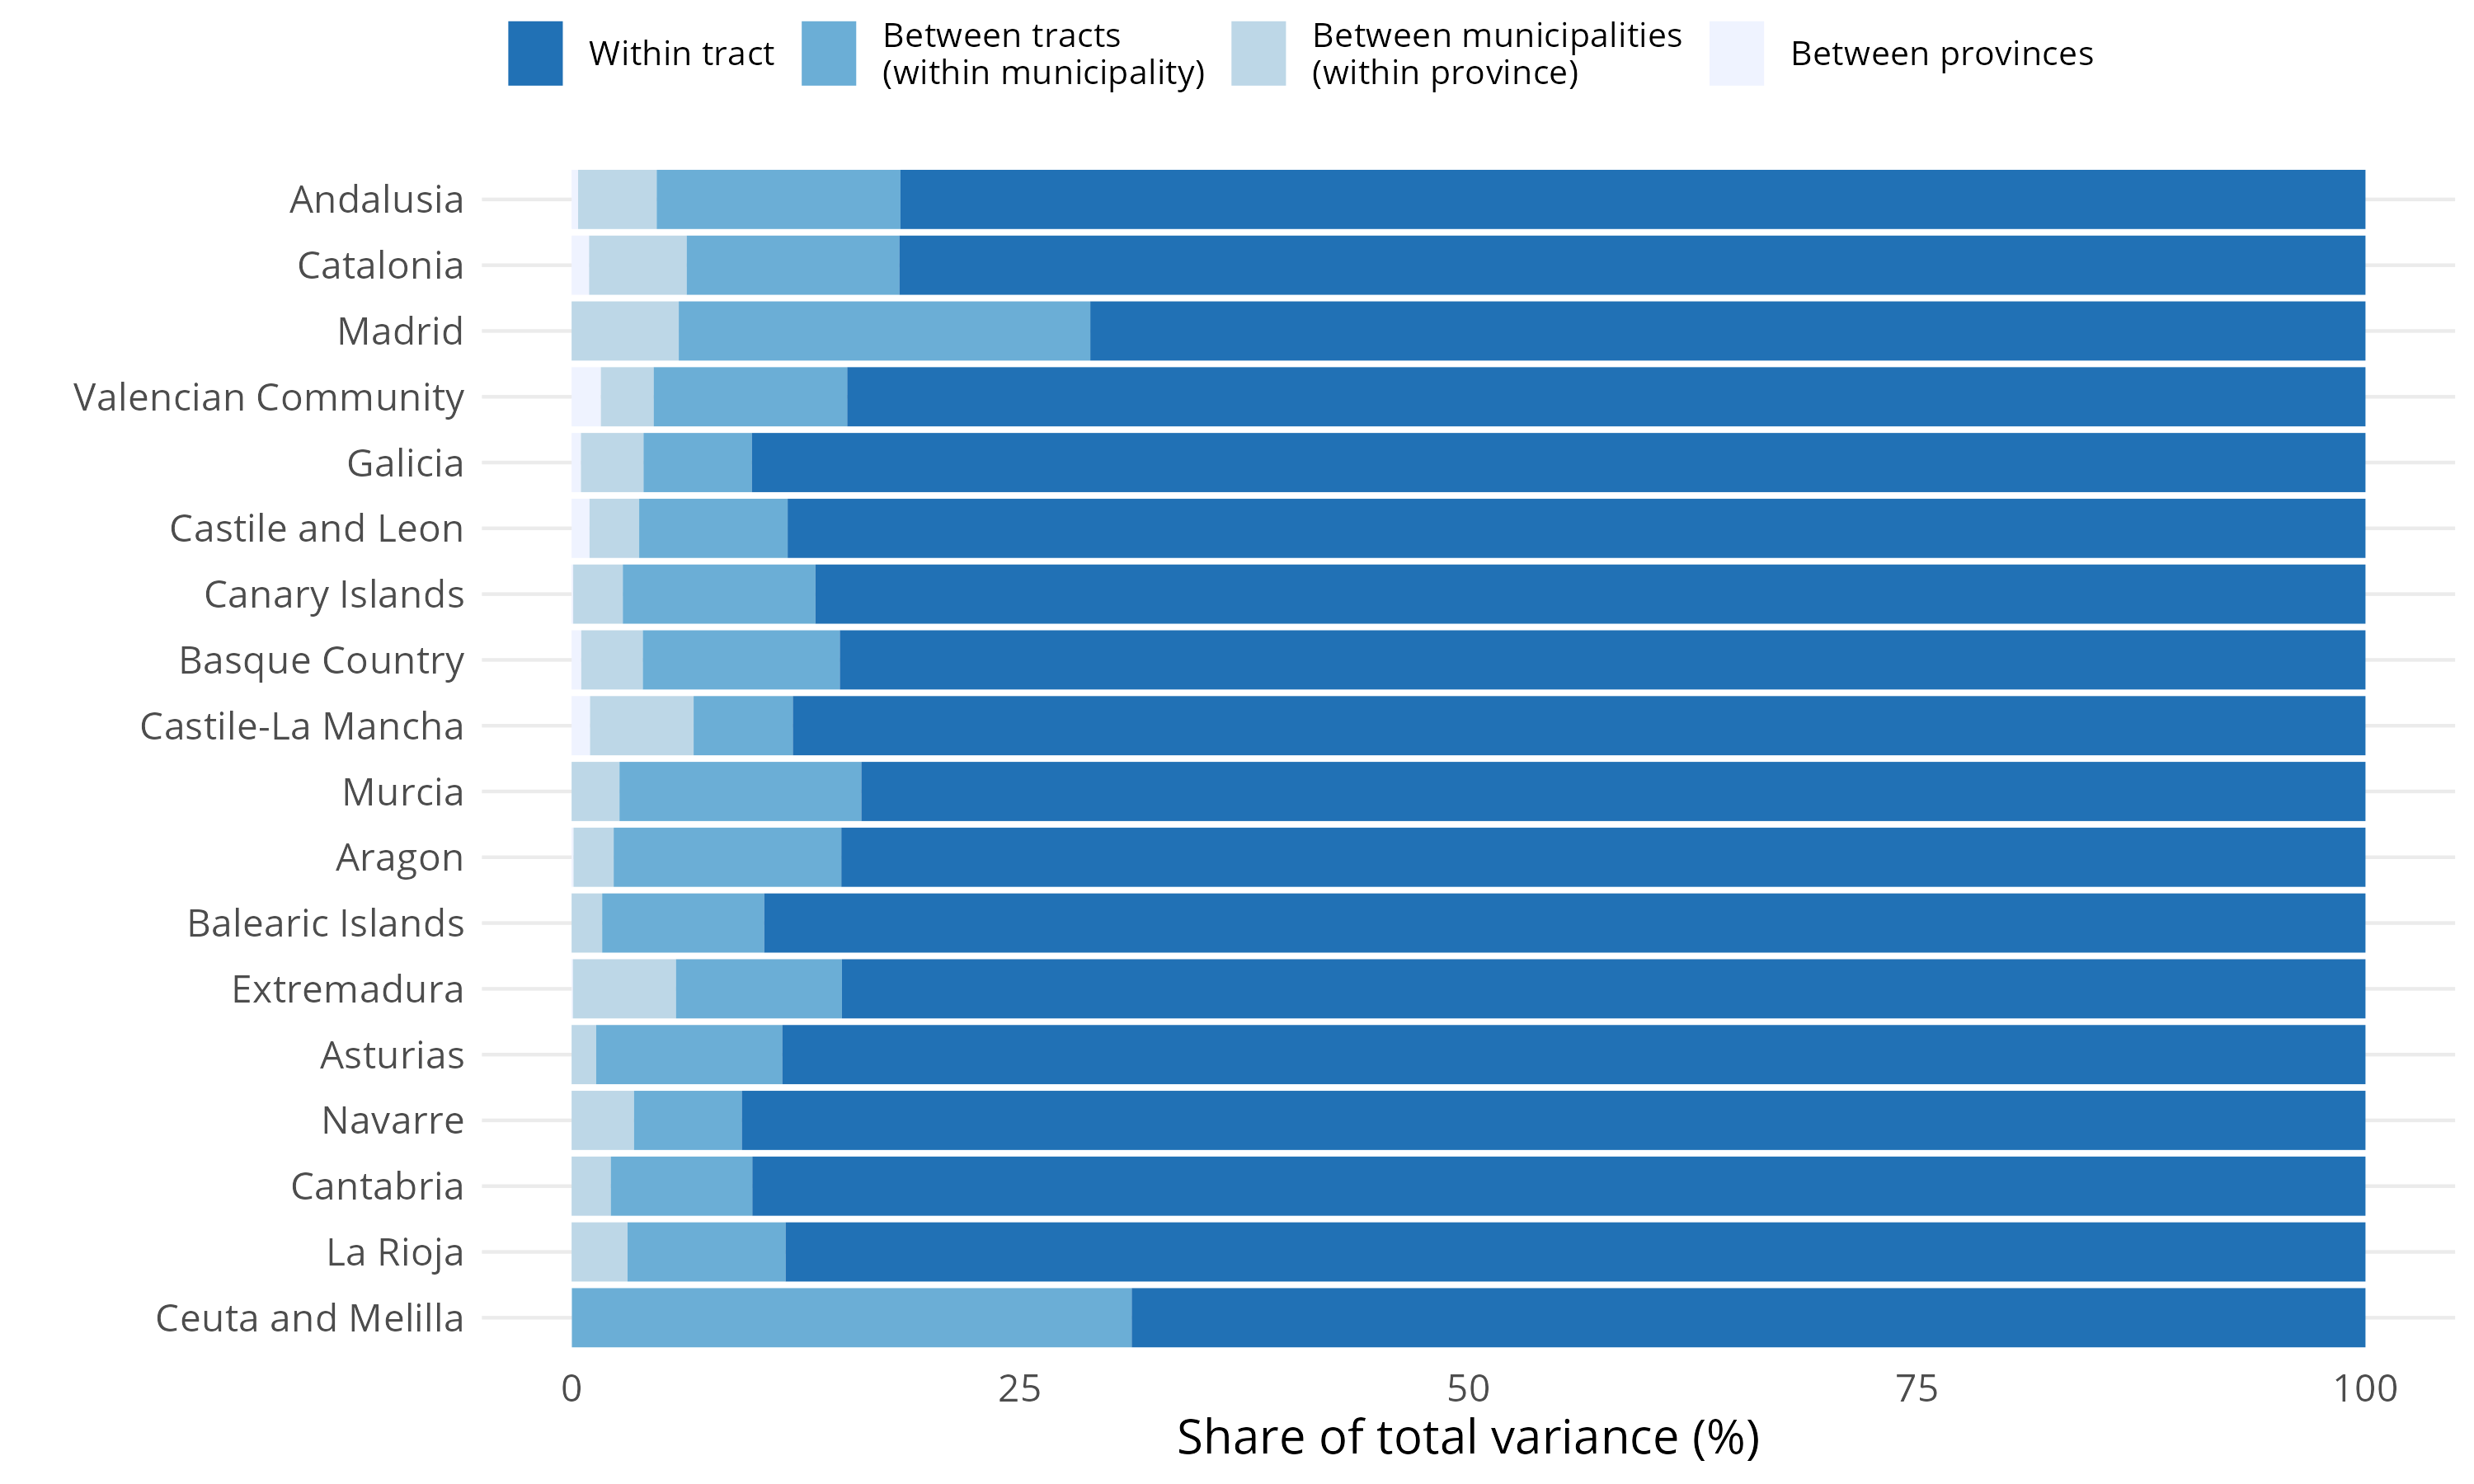
\includegraphics[width=0.9\textwidth]{output/variance_decomp.png}
\end{center}
\begin{fignotes2}
\textbf{Notes:} This figure shows the decomposition of total variance in log income into four components: within-tract, between-tract (within municipality), between-municipality (within province), and between-province variation. The within-tract component is calculated assuming log-normality within tracts, while the remaining components are computed using population-weighted variance decomposition. Regions are ordered by total population. Source: Spanish Statistical Office and author's calculations.
\end{fignotes2}
\end{figure}